\subsection{Interaction analysis}

The software Trentool (\cite{3.4.Trentool}, version 3.3.2, 6th June 2015) was used with Matlab 2013a for exploring entropy transfers between cortical areas.
The procedure consisted of three sections: Preparation, transfer entropy calculation and evaluation of the results.

\paragraph{Preparation}
First, the input datasets were prepared for the analysis.
This dataset consisted of three parts: regional activity from single trials, a list of regional connections and a set of parameters.

To create the first dataset part, two sets of single trials (one for each condition) were selected from each subject.
For this step, cortical regions were selected if they showed syntax effects either in the cluster analysis or the interval analysis.
This process yielded six relevant cortical regions: PAC, aSTG, pSTS, BA44, BA45 and BA6v.
Mean activity from these regions was lowpass filtered with a digital, single-pass FIR filter \footnote{passband frequency of 250Hz, stopband frequency of 300Hz, ripple of 1db, stopband attenuation of 120db; implemented with the \emph{filter} function in Matlab} to suppress the influence from the HPI coils.
This filter introduced a signal lag of 79ms, and selected time windows were shifted accordingly.

To create the second dataset part, I examined which were the most relevant functional connections between cortical regions.
There are 720 unique possiblities to compare the previously mentioned six regions, which would overwhelm\footnote{The comparison over one pair of cortical regions, in forward and reverse directions, over two conditions and 50 separate shift delays, required a computation time of 35 CPU cores * hours per subject and timewindow. Calculating transfer entropy between 36 pairs of regions took a total of 3150 CPU cores * hours, which - thanks to the work of Christian Labadie and Hermann Sonntag - amounted to 48 actual hours of calculation time. The task of computing the full set of 720 comparisons would have required 63000 CPU cores * hours - for other groups, a sufficient reason to switch a GPU-based algorithm\cite{3.4.gpuTE}.} the computational capacity at my disposal and yield a large proportion of meaningless results.
For these reason, I limited the calculation to comparisons between regions along the same axonal fiber bundle.

I selected comparisons between all language-related regions along three pathways (see Fig. \ref{3.4.regions}) that are known to be involved in subject-object-paradigms.
The following regions associated to each pathway are derived from \cite{1.1.pathways}.

The second dorsal language pathway, via the arcuate fascicle, connects the regions PAC, pSTG and BA44.
This pathway is therefore represented by two short connections ($PAC_{lh} \rightarrow pSTG_{lh}$ and $pSTG_{lh} \rightarrow BA44_{lh}$) and one long connection ($PAC_{lh} \rightarrow BA44_{lh}$).

The second ventral language pathway, via the inferior fronto-occipital fascicle, connects the regions PAC, aSTG and BA45.
This layout yields two short connections ($PAC_{lh} \rightarrow aSTG_{lh}$, $aSTG_{lh} \rightarrow BA45_{lh}$) and one long connection, $PAC_{lh} \rightarrow BA45_{lh}$.

The first dorsal language pathway, via the nomen nescio and the third component of the superior longitudinal fascicle, connects the regions pSTG, SMG and BA6v.
SMG is a substantially larger region than pSTG and BA6v, and is apparently responsible for sensory integration.
Task-related effects tend to disappear when averaging over large regions, even when these regions are primarily involved in task-related processing.
Due to this effect, and the minimal role of SMG in object-subject paradigms, I decided to skip the connections $pSTG_{lh} \rightarrow SMG_{lh}$ and $SMG_{lh} \rightarrow BA6v_{lh}$ in the signal transfer calculations.
Consequently, the motor component of the language network will be represented by the long connection $pSTG_{lh} \rightarrow BA6v_{lh}$.

The analysis included two functional regions (BA44/BA45 and aSTG/pSTG) that share a common gyrus.
Since gyri are highly interconnected, a certain degree of information exchange can be expected.
Connections between those regions were examined as well, yielding another two short connections ($BA44_{lh} \rightarrow BA45_{lh}$ and $aSTG_{lh} \rightarrow pSTG_{lh}$).

In order to compute forward and backward directions, two separate calculations are necessary for each comparison.
Therefore, examing the information transfer along these nine regional connections requires 18 sets of calculations.

\begin{figure}[h]
\begin{center}
\vspace{7mm}
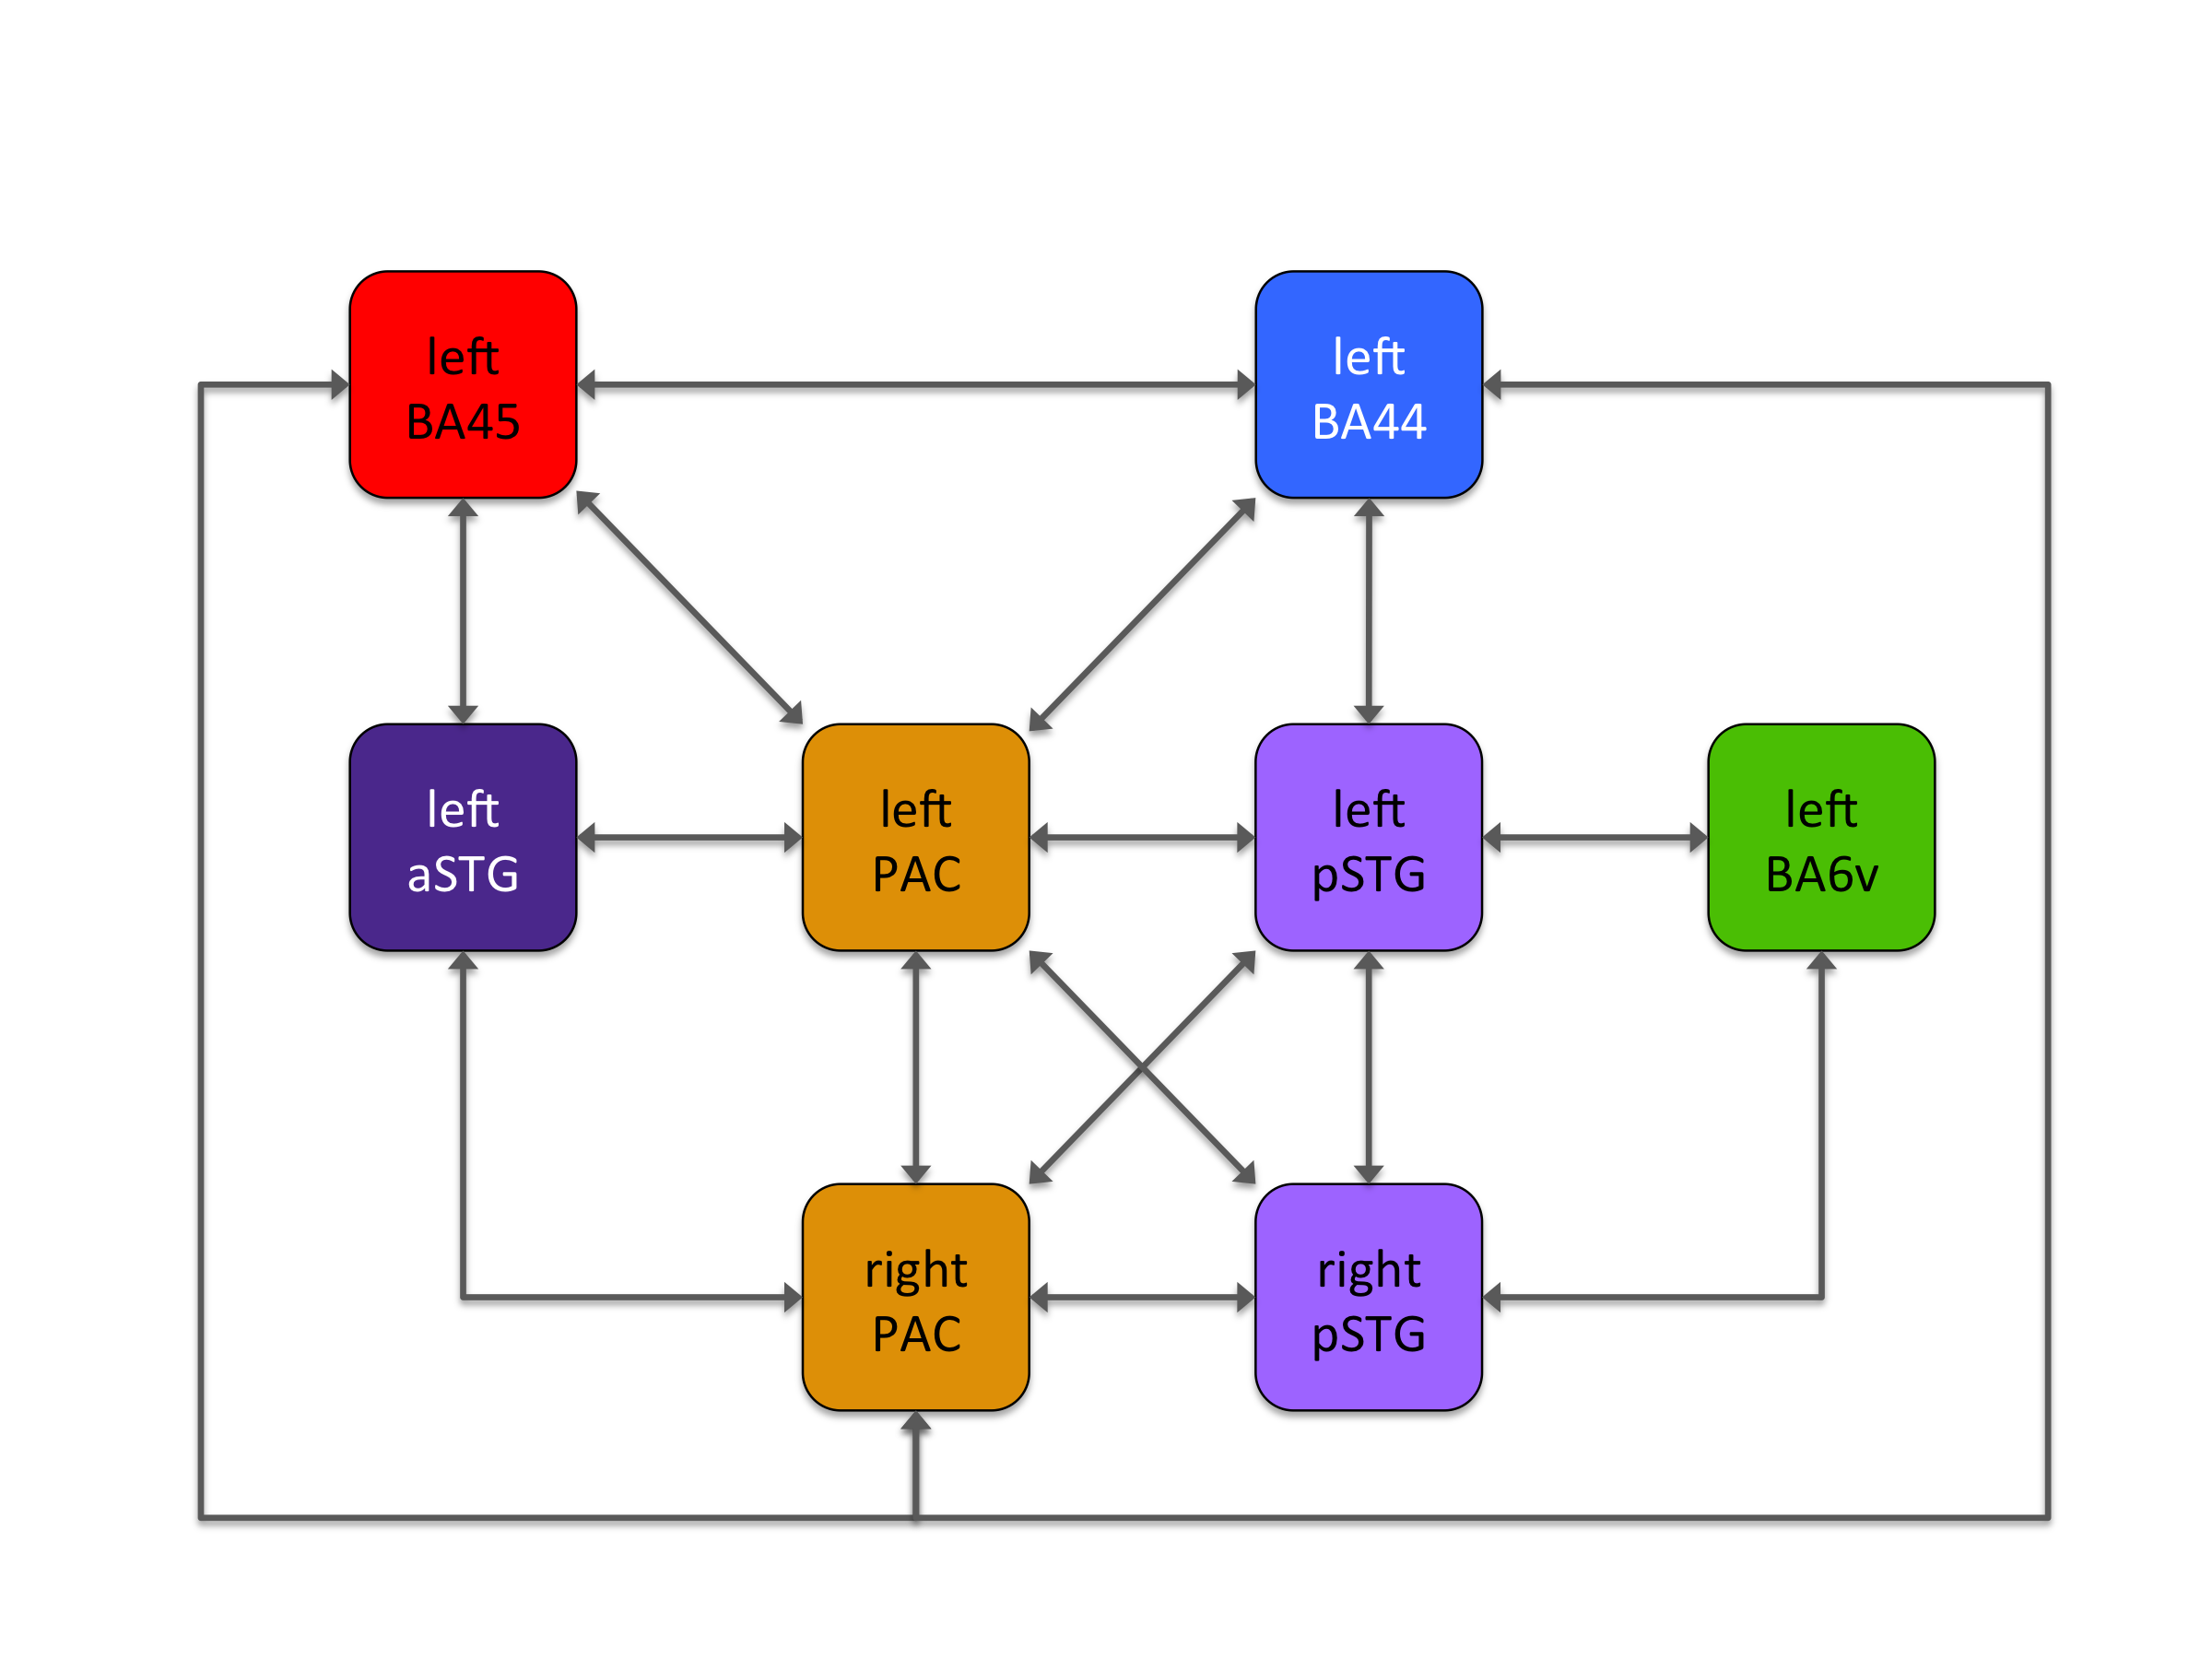
\includegraphics[width=0.75\textwidth]{pics/3_4_regions.png}
\caption{\label{3.4.regions} Connections of selected cortical regions for the computation of transfered entropy.}
\end{center}
\end{figure}

To create the third dataset part, I selected a set of parameters for the data preparation.

First, I needed to define a time interval that is analyzed for transfer entropy.
The interval analysis showed (see chapter \ref{4.3}) that syntax effects occurred predominantly up to 1000ms after onset.
These effects were based on group analysis, while the following interaction analysis was based on a single-subject, single-trial analysis.
Due to these circumstances, I decided against limiting the interaction analysis to the previously discovered time intervals, and for exploring the full time range between 0ms and 1000ms (after stimulus onset) instead.
As a reasonable tradeoff between time resolution and data content, I fragmented the analysis into five segments of 200ms.

Next, I needed to choose embedding parameters.
To understand embedding, it is important to know that the transfer entropy estimation fundamentally relies on the comparison between two probability density functions.
These mathematical constructs can only be approximated from scalar time series.
For this purpose, time series from individual trials are combined into a multidimensional state space by Trentool.
The reduction of this multidimensional space into a probability density function is the process called embedding.
There are four important embedding parameters: the embedding criterion, the embedding time, the embedding delay range and the embedding dimension range.

For choosing suitable parameter ranges, I followed the recommendations described in the Trentool tutorial \cite{3.3.TrentoolTutorial}.
As for the embedding criterion, I selected the Ragwitz criterion (\emph{cfg.optimizemethod = 'ragwitz'}).
It is recommended for EEG/MEG data, while the only other option - the Cao Criterion - is recommended for fMRI data.

The embedding delay is denominated in multiples of the autocorrelation time (ACT).
The embedding setup relies heavily on this metric.
The ACT is defined as the first positive minimum of the self-correlation of the signal.
For my set of single trials, the median ACT was 2ms (90th: 6ms, 95th: 10ms, 99th: 22ms, 99.9th: 34ms).
The usable embedding interval depends on the maximum ACT, but the embedding interval must be identical for all datasets.
Hence, a single trial with a high ACT can reduce the effective embedding interval for all other trials.
I set the parameters \emph{cfg.trialselect = 'ACT'} and \emph{cfg.actthrvalue = 12} so that trials with an ACT greater than 12 were excluded from the analysis.
This setting caused a rejection of 3.4\% of all trials.
The relatively high rejection rate was required to ensure that the maximum embedding interval wouldn't exceed 1000 samples in combination with the following embedding delay and embedding dimension.

As recommended, I set the embedding delay to a search range between 0.2 and 0.5 times of the autocorrelation delay, (\emph{cfg.ragtaurange = 0.2:0.5}).
A preliminary analysis with a embedding dimension range of 2 to 12 yielded 12 as the most common embedding dimension, indicating a ceiling effect.
To alleviate this ceiling effect, I extended the maximum embedding dimension by two (\emph{cfg.ragdim = 7:14}).

For the embedding process, a considerable section of data is necessary to estimate the baseline entropy before the interaction time cue occurs.
This section of data is referred to as embedding time, and won't be included in the analysis of transfer entropy.
It is necessary to define the embedding time and TOI with a combination of two variables, \emph{cfg.toi} and \emph{cfg.repPred}.
repPred denominates the length of the TOI that is actually used for the information transfer calculation.
With a sampling rate of 1000 samples per second and a desired time window of 200ms, I set it to \emph{cfg.repPred = 200}.
Due to an implementation quirk in Trentool, selecting a fixed data interval for the signal transfer calculation is not possible\footnote{According to the comment section of \emph{transferentropy.m}: ``The span of time needed for embedding is: (max(dim)-1)*max(tau). The prediction time starts after this embedding time. Hence the span of time defined in cfg.toi must be a good deal longer than the embedding time, at least embedding time plus 150 samples or max(cfg.predicttime\_u).``
Since tau depends on ACT, which in turn is different for each data set, it is impossible to compute a fixed embedding time for all data sets.}. The Trentool authors expect their users to set a very broad TOI, leaving enough samples to both include the relevant data and the embedding time in all cases.
This implementation leads to a sliding TOI (fixed length, but with varying onset) for the actual information transfer calculations.
Since the intention was to explore signal interactions at clearly defined time intervals, the Trentool implementation was too imprecise for my goals.
In order to achieve a higher degree of control across trials and subjects, I modified the routine \emph{transferentropy.m} (for a detailed explanation, see \ref{Appendix.A}) to use a fixed TOI for its calculations.
With this modification, Trentool adapted the start - instead of the end - of the internal data interval dynamically to the length of the embedding interval.
To achieve this effect, \emph{cfg.toi} was set to the start and end of the TOI, plus a fixed filter delay of 79ms.
\emph{cfg.repPred} was set to the length of the TOI in samples, i.e., 200.

Using this dataset, Trentool used the Ragwitz criterion to optimize the embedding parameters for each collection of trials.
This process was repeated for each subject, time window and condition.
The most common optimal embedding dimension was 14 (minimum: 12).

After the individual parameter optimization, the process was repeated to prepare the datasets for group comparisons.
Originally, this process was intented to be conducted by the function \emph{TE\_groupprepare}.
Since this function was designed to run on a single computer (requiring a calculation time of more that 50 hours in this case), I replaced it with an equivalent routine that allowed distributed computing (see \ref{Appendix.A}).

\paragraph{Transfer entropy calculations}

After embedding, Trentool performed an interaction shift test.
This procedure (performed with the function \emph{InteractionDelayReconstruction\_calculate}) counteracts bias introduced by noise, especially the common false positive detection of an interaction between two data sets with different signal-to-noise levels.
The shift test establishes the optimal delay of transfered entropy for each comparison of activity.
Transfer entropy was computed for a time range of possible interaction delays: 1ms to 50ms in steps of 1ms.
Trentool then selected the interaction delay with the biggest associated transfer entropy as the most likely representation of the signal delay caused by cognitive processes and anatomic constraints.
To alleviate issues with volume conduction, I supplied the option \emph{cfg.extracond = 'Faes\_method'}.
Unfortunately, using this method prevents the determination of the precise signal delay.
Since the signal delay is not relevant to my research goals, this trade-off was trivial to solve.
The optimal dimension for each data set was considered with the option \emph{cfg.optdimusage = 'indivdim'}.

During testing for the impact of experimental conditions, real effects are commonly confounded with spurious effect due to random differences.
To counteract this issue, Trentool offers the creation of surrogate data.
This possibility allows for comparing transfer entropy between real and surrogate data, rather than between conditions.
The surrogate data was created by shuffling existing trials (\emph{cfg.surrogatetype = 'trialshuffling'}).
The significance level for this procedure was 1\% (\emph{cfg.alpha = 0.01}).
I used t-values to represent the statistical results of the shift test (\emph{cfg.permstatstype = 'indepsamplesT'}).
These results indicated the likelihood if an entropy transfer has occurred between the selected pair of regional activity.

If three or more significant interactions were detected within a single dataset, the results were corrected for cascade effects and simple common mode drive effects with the Trentool function \emph{TEgraphanalysis}.
The detection threshold was 3ms (\emph{cfg.threshold = 3}) and I used FDR-uncorrected probability values to select signficant interactions (\emph{cfg.cmc = 0}).

\paragraph{Result evaluation}

I combined these subject-level results in Matlab to obtain group-level results.
As suggested by \cite{3.4.binomialtest}, I performed a binomial test (implemented in Matlab with the function \emph{binofit}) to examine whether more significant results (p < 5\%) occur than expected when assuming that the null probability of a significant result is 5\%.
This probability was corrected for multiple comparisons \cite{3.4.FDR.a} with the Matlab function \emph{fdr\_bh} with an alpha of 5\% \cite{3.4.FDR.implementation}.
Furthermore, I estimated the extent of transfer entropy for every functional connection by calculating a  mean across all subjects.
For calculating the mean transfer entropy, only interactions were considered that passed the surrogate test.

Finally, I evaluated the impact of the syntax condition on all subjects.
For this group-level comparison, a clustered T-test compared transfer entropy between conditions over all subjects by using the Trentool function \emph{TEgroup\_stats}.

A separate comparison was conducted for each of the five timewindows.